\documentclass[
	digital, oneside, nosansbold, nocolorbold, nolot, nolof
]{fithesis4}

\usepackage[resetfonts]{cmap}
\usepackage[T1]{fontenc}
\usepackage[english]{babel}
\usepackage[utf8]{inputenc}

\thesissetup{
    date        = \the\year/\the\month/\the\day,
    university  = mu,
    faculty     = fi,
	department  = {Department of Machine Learning and Data Processing},
    type        = mgr,
    author      = Šimon Varga,
    gender      = m,
    advisor     = {prof. RNDr. Luboš Brim, CSc.},
    title       = {%
		Influence maximization in partially specified Boolean networks},
    keywords    = {keyword1, keyword2, ...},
    abstract    = {%
      This is the abstract of my thesis, which can

      span multiple paragraphs.
    },
    thanks      = {%
      These are the acknowledgements for my thesis, which can

      span multiple paragraphs.
    },
    bib         = bib.bib,
    facultyLogo = fithesis-fi,
}

\usepackage{makeidx}      %% The `makeidx` package contains
\makeindex                %% helper commands for index typesetting.
%% These additional packages are used within the document:
\usepackage{mathtools}
\usepackage{amsthm}
\usepackage{amssymb}
\usepackage{amsfonts}
\usepackage{IEEEtrantools}
\usepackage{subcaption}
\usepackage{tikz}
\usetikzlibrary{shapes, positioning}
\usepackage{url}      %% Hyperlinks
\usepackage{listings} %% Source code highlighting
\lstset{
  basicstyle      = \ttfamily,
  identifierstyle = \color{black},
  keywordstyle    = \color{blue},
  keywordstyle    = {[2]\color{cyan}},
  keywordstyle    = {[3]\color{olive}},
  stringstyle     = \color{teal},
  commentstyle    = \itshape\color{magenta},
  breaklines      = true,
}
\usepackage{floatrow} %% Putting captions above tables
\floatsetup[table]{capposition=top}
\usepackage[babel]{csquotes} %% Context-sensitive quotation marks


\theoremstyle{definition}
\newtheorem{definition}{Definition}

\theoremstyle{definition}
\newtheorem{example}{Example}

\newenvironment{ldefinition}
    {\begin{definition}}
	{\par\hspace{\stretch{1}}$\spadesuit$\hspace{\stretch{1}}
     \par\end{definition}}

\newenvironment{lexample}
    {\begin{example}}
    {\par\hspace{\stretch{1}}\rule{0.2\textwidth}{0.01ex}\hspace{\stretch{1}}
     \par\end{example}}


\DeclareMathOperator{\stg}{stg}

\NewDocumentCommand{\BN}{m}{\mathcal{#1}}
\NewDocumentCommand{\BNRs}{m}{\mathcal{#1}} % BN Regulations
\NewDocumentCommand{\BNUFs}{m}{\mathcal{#1}} % BN Update Functions
\NewDocumentCommand{\state}{m}{\mathtt{#1}} % State (for triplets 101, ...)
\NewDocumentCommand{\attr}{m}{\mathcal{#1}} % Attractor

\NewDocumentCommand{\BNt}{m}{\to_{\BN{#1}}} % BN transition
\NewDocumentCommand{\BNtc}{m}{\rightsquigarrow_{\BN{#1}}} % transitive closure

\NewDocumentCommand{\dset}{m}{\mathfrak{#1}} % driver set

\NewDocumentCommand{\dom}{m}{\mathcal{D}(#1)} % domain

\DeclarePairedDelimiter{\set}{\{}{\}}



\begin{document}

\chapter{Introduction}

\paragraph{Systems biology}

A common trait among all humans is a desire to know, to understand. Aristotle
(384--322~BC) described this desire in his work Metaphysics~\cite{aristotle}:

\blockquote[Aristotle]{All men by nature desire to know. An indication of this
    is the delight we take in our senses; for even apart from their usefulness
    they are loved for themselves; and above all others the sense of sight. For
    not only with a view to action, but even when we are not going to do
    anything, we prefer sight to almost everything else. The reason is that
    this, most of all the senses, makes us know and brings to light many
    differences between things.}

A human ambition to see, to explore the world around and inside us has emerged
into many sciences -- one of them being biology, a scientific study of life.
There is a visible trend of \emph{reductionism} interweaving the history of
biology. In the 17th century, René Descartes (1596--1650) stated that complex
systems could be understood by looking into the smaller parts inside the system
and then reassembly them into the whole. Although biology has not yet existed
back then as a scientific discipline of today and the main areas affected by
Descartes' idea of reductionism were mathematics and physics, he also published
his notion of non-human animals being complex automatons designed by a God. He
claimed that such an automaton can be described in a reductionist and
mechanistic way.~\cite{systems_bio_hist, de_homine}

A change in this concept arose in the early part of the 20th century. An
influential work by Norbert Wiener (1894--1964) asked for more system-level
understanding~\cite{cybernetics}.  Many biologists expressed objections against
reductionist attitudes~\cite{woodger_biological, weiss_problem, ludwig_open}. A
new language was used, with dominant terms like complexity, organization,
uniqueness, emergence, unpredictability, and interconnectedness. Reductionistic
and mechanistic biology lacks a view of the vital orchestration of components.
Against reductionism, another paradigm started to be articulated more --
\emph{holism}, coined by Jan Smuts (1870--1950), naturalist, philosopher, and
twice Prime Minister of South Africa~\cite{smuts_holism}.

Although these two theories -- reductionism and holism -- are often put in
contrast to each other, no opposition but reconciliation is needed. It is
important to explore the smaller subsystems, tiny components, and how they
function on their own (reductionism). However, it is not less important to look
at the system from above to explore possible emergent features resulting from
the interplay between components (holism).~\cite{systems_bio_hist}

A nice example is an aggregate motion of a flock of birds.
Reynolds~\cite{reynolds_flock} published a computer simulation where each
agent-bird behaves accordingly to a relatively simple set of rules. A
reductionist scientist could explore these rules and understand the bird's sole
behavior but could not find any evidence among the rules of the amazing
phenomenon because it emerges from the interactions between the components
(birds). A set of simple rules orchestrating the components emerged in the
complex behavior of the whole system -- this is something central to a new
approach in biology rising from holism: \emph{Systems biology}.

To study even a small entity -- a cell -- from the system-wide perspective, one
has to combine interactions of many components on different levels: genome,
transcriptome, proteome, and metabolome space. Processing such a huge amount of
information requires computational methods and software infrastructure,
critical components for systems biology research.~\cite{kitano_overview,
systems_bio_methods}

\paragraph{Boolean networks}

Systems biology models of living systems' dynamics may be categorized as
qualitative or quantitative. An example of a qualitative model is a set of ODE
(ordinary differential equations) precisely describing the kinetics of
processes in the system. Experimental inference of all the kinetic parameters
is usually a complex task. At this place, systems biology benefits from
qualitative models. This work targets one concrete: \emph{Boolean networks}
(BN). BN is a simple model introduced by Stuart Kauffman in 1969 for genetic
regulatory networks (GRN), consisting of simple boolean variables for
components of the GRN (proteins, genes, and metabolites) and discrete relations
between them.  Each variable represents the component being active or not. If
the component is a gene, then the variable represents whether the gene is
transcribed or not. In the case of metabolites or proteins, it may represent
whether the amount of metabolite or protein is sufficient for some reaction.
Boolean functions define the relations between the
variables.~\cite{concepts_bn} Even after such a modeling reduction from the
real-world living system, BNs still may illustrate various processes such as
heart development~\cite{heart_development} and aging of organisms~\cite{aging}.

BNs play an important role in systems biology, but it is often hard to infer
the boolean functions controlling the system. A knowledge that some protein
\(a\) and \(b\) activate another protein \(c\) is insufficient because both
boolean functions \(a \land b\) and \(a \lor b\) are consistent with the
knowledge. This uncertainty may be expressed in a \emph{parametrised boolean
network} (PBN), a more general version of BN.

\paragraph{Attractors and control}

One crucial question about any system is: \enquote{How will the system look
after a long time? Will it settle and not change anymore?} The state the system
will eventually evolve into and never leave is called an \emph{attractor}. Such
a state does not have to be single; an attractor may also consist of multiple
states. In that case, the system switches among the states and visits each
infinitely often, but again, only those states in the attractor, no others.. In
the context of systems biology, an attractor is called a \emph{phenotype} as
well.

Finding a control strategy that drives the system to a desired attractor is
beneficial for many applications, for example, identifying key therapeutic
targets for controlling pathways of regulatory and signaling networks,
providing a basis for designing \emph{in vitro} cell reprogramming experiments,
and many more~\cite{control_psbn}. It is known that this problem is
\(\mathcal{NP}\)-hard in general for boolean networks, but effective
approximations exist ranging from linear to cubic time
complexities~\cite{control_akutsu}. Last year, T.~Parmer et~al. presented an
article~\cite{infl_max_BN} with a novel approximation approach based on a
well-studied problem of \emph{influence maximization} for spreading processes
in social networks.

\paragraph{Our contribution}

The last cited article about influence maximization became a stimulus for this
thesis. T.~Parmer later published
\cite{parmer_dynamical}~and~\cite{parmer_phd}, elaborating more on influence
and control in network-based models. However, to the best of our knowledge, no
attempt to generalize to parametrized boolean networks has been published yet.
Thus, in this work, we aim to adjust their idea to work with PBNs, benchmark on
a suitable set of networks, and design a simple, user-friendly GUI to analyze
models of the user's choice.


\chapter{Preliminaries}

This chapter provides theoretical background related to our work, all the
definitions with examples to facilitate understanding, and the final problem
formulation. For a more in-depth description, we refer a reader to other
articles: for boolean networks~\cite{concepts_bn}, for parametrized
BNs~\cite{kadlecaj_thesis}, and finally for controlling BNs~\cite{infl_max_BN}.
The definitions and notions in our work are adopted from those articles.

\section{Boolean network}

The introduction chapter presented boolean networks in an informal, intuitive
way. Now, we show a solid mathematical definition here.

\begin{ldefinition}
A \emph{boolean network} is a 3-tuple $\BN{B} = (V, \BNRs{R}, \BNUFs{F})$,
where:
\begin{description}
\item[$V = \{a, b, c, \ldots \}$] stands for a finite set of
    \emph{boolean variables}, which take on values from $\set{0, 1}$.
\item[$\BNRs{R} \subseteq V^2$] is a set of regulations $(a, b)$. We write
    that the variable $a$ \emph{regulates} the variable $b$, meaning $a$
    appears in the update function for $b$. \emph{Context} of a variable
    $a$ is a set of its regulators
    \[C_{\BN{B}}(a) = \set{b \mid (b, a) \in \BNRs{R}}\]
    We write just $C(a)$ instead of $C_{\BN{B}}(a)$, when it is unambiguous.
\item[$\BNUFs{F}$] is a total mapping from $V$ to a set of
    \emph{update functions}. An update function for variable $v \in V$ is
    denoted as $\BNUFs{F}_v$ and takes a value of every variable in $v$'s
    context as an input and outputs an \emph{update value} for the variable
    $v$.
    \[
        \BNUFs{F}_v \in \set*{F \mid F: \set{0, 1}^{C(a)} \to \set{0, 1}}
    \]
\end{description}
\end{ldefinition}

\begin{lexample} \label{example:BN}
In this example we illustrate the previous definition for a simple 3-variable
boolean network depicted in figure~\ref{fig:bn}.
\begin{figure}[!ht]
\centering
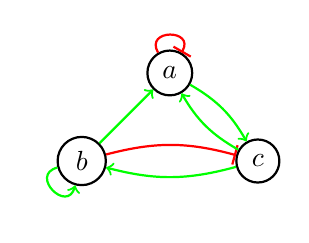
\begin{tikzpicture}[node distance={4.5em}, thick, main/.style = {draw, circle}] 
    \node[main] (a)                        {$a$}; 
    \node[main] (b) [below left of=a]       {$b$};
    \node[main] (c) [below right of=a]        {$c$};

    \draw[red, -|] (a) to [out=120, in=60, looseness=3] (a);
    \draw[relative, green, ->] (a) to [out=15, in=165, looseness=1] (c);

    \draw[green, ->] (b) -- (a);
    \draw[green, ->] (b) to [out=195, in=255, looseness=3] (b);
    \draw[relative, red, -|] (b) to [out=15, in=165, looseness=1] (c);

    \draw[relative, green, ->] (c) to [out=15, in=165, looseness=1] (a);
    \draw[relative, green, ->] (c) to [out=15, in=165, looseness=1] (b);
\end{tikzpicture}
\caption[An example of a BN]{An example of a regulatory graph of a boolean
network. The directed graph is given by the variables and the regulations of
the BN. Here, the edges are moreover colored according to the effect in the
corresponding update function.\label{fig:bn}}
\end{figure}

Clearly, the network contains three boolean variables $\set{a, b, c}$ and
regulations between them:
\[
    \BNRs{R} = \set{(a, a), (a, c), (b, a), (b, b), (b, c), (c, a), (c, b)}
\]

We can define the update functions in multiple ways to be still consistent with
the figure~\ref{fig:bn}. By \enquote{consistent} we mean that for each
regulation $(x, y)$ colored green (red), for every possible valuation of the
other regulators of $y$, changing $x$'s value from 0 to 1 does not change the
value of $\BNUFs{F}_y$ from 1 to 0 (0 to 1, resp.). One of the consistent
definitions is:
\begin{IEEEeqnarray*}{rCl}
    \BNUFs{F}_a(a, b, c) & = & \lnot a \land b \land c\\
    \BNUFs{F}_b(   b, c) & = & b \land \lnot c\\
    \BNUFs{F}_c(a, b   ) & = & a \lor \lnot b
\end{IEEEeqnarray*}

To be more precise in terms of the previous definition, we should write
$\BNUFs{F}_a(\nu) = \lnot \nu(a) \land \nu(b) \land \nu(c)$ instead of
$\BNUFs{F}_a(a, b, c)$ because an update function takes a mapping $\nu: C(a) \to
\{0,1\}$ as a parameter and not the variables $C(a)$ directly. We omit this one
level of indirection for the sake of fluency when reading.

Update functions can also be defined by truth tables:
\[
\begin{array}{ccc|c}
    a & b & c & \BNUFs{F}_a\\
    \hline
    1 & 1 & 1 & 0\\
    1 & 1 & 0 & 0\\
    1 & 0 & 1 & 0\\
    1 & 0 & 0 & 0\\
    0 & 1 & 1 & 1\\
    0 & 1 & 0 & 0\\
    0 & 0 & 1 & 0\\
    0 & 0 & 0 & 0\\
\end{array}
\qquad
\begin{array}{cc|c}
    b & c & \BNUFs{F}_b\\
    \hline
    1 & 1 & 0\\
    1 & 0 & 1\\
    0 & 1 & 0\\
    0 & 0 & 0\\
\end{array}
\qquad
\begin{array}{cc|c}
    a & b & \BNUFs{F}_c\\
    \hline
    1 & 1 & 1\\
    1 & 0 & 1\\
    0 & 1 & 0\\
    0 & 0 & 1\\
\end{array}
\]
\end{lexample}

A BN describes the system structure: main components, and their interactions.
Then, the system evolves and changes its \emph{state} over time according to the
interaction rules -- update functions.

\begin{ldefinition}
A \emph{state} of a boolean network $\BN{B}$ with variables $V$ is a
(total) valuation $\nu : V \to \set{0, 1}$.
\end{ldefinition}

\subsection{Dynamic behavior of boolean networks}

A BN update functions together with \emph{semantics} specifies possible
transitions between states. BN semantics is an \emph{updating policy} for
applying the update functions to a BN's state. There is a wide space for such
policies: the two most common, \emph{synchronous} and \emph{asynchronous}, but
others more sophisticated, synchronous block-sequential, stochastic
asynchronous, and more~\cite{colomoto}. In synchronous semantics, all the
update functions are applied at once. In the asynchronous, only one update
function is used at a time. It was thought that the latter represents
biological systems better, as the components in a living system usually have
concurrent dynamics. Conversely, synchronous updating policy leads to fewer
transitions, and some discussion revealed that it might be more appropriate for
robustness analysis~\cite{concepts_bn}. We made a choice for synchronous
semantics mainly because of the stimulating paper of T.~Parmer~et~al., where
the authors aimed for that policy the most~\cite{infl_max_BN}.

\begin{lexample}
Continuing with the BN from example~\ref{example:BN}, we compare the two most
frequent semantics regarding state $\state{110}$. We write triplet
$\state{110}$ instead of more complex, formal valuation $\set{(a, \state{1}),
(b, \state{1}), (c, \state{0})}$. Asynchronous semantics have two possible
consequent states: $\state{010}$ (after application of $\BNUFs{F}_a$) and
$\state{111}$ ($\BNUFs{F}_c$).  Synchronous semantics have only one:
$\state{011}$.
\end{lexample}

After intuitively describing what semantics is, we provide a definition of
synchronous semantics here:
\begin{ldefinition}
A boolean network $\BN{B} = (V, \BNRs{R}, \BNUFs{F})$ can transition from a
state $\nu_{\text{fr}}$ to a state $\nu_{\text{to}}$ in \emph{synchronous
semantics} if and only if:
\[
    \forall_{v \in V} : \BNUFs{F}_v(\nu_{\text{fr}}\restriction C(v)) =
    \nu_{\text{to}}(v)
\]
Where $\nu\restriction C(v)$ is a restriction of $\nu$ to the domain $C(v)$.

We also define a relation $\BNt{B}$ of feasible transitions, consisting of
all the pairs $(\nu_{\text{fr}}, \nu_{\text{to}})$ such that $\BN{B}$
can change state from $\nu_{\text{fr}}$ to $\nu_{\text{to}}$. We use the notions
$(\nu_{\text{fr}}, \nu_{\text{to}}) \in \BNt{B}$ and
$\nu_{\text{fr}} \BNt{B} \nu_{\text{to}}$ interchangeably.

A transitive closure of $\BNt{B}$ is denoted $\BNt{B}^* = \BNtc{B}$.
\end{ldefinition}

The dynamics of a boolean network can be interpreted as a directed
graph\footnote{\url{https://en.wikipedia.org/wiki/Directed_graph}}, where the
vertices correspond to the states of a BN, and the arcs correspond to the
feasible transitions for a given semantics. The number of vertices is
exponential ($2^{|V|}$) with respect to the number of BN variables because each
variable may (independently) take on two values from~$\set{0, 1}$. There is
always just one outgoing arc from any node for synchronous semantics. From now
on, we consider only synchronous update policy, except we mention the semantics
explicitly.

\begin{ldefinition}
A \emph{state transition graph} (STG) of a BN $\BN{B} = (V, \BNRs{R},
\BNUFs{F})$ is a directed graph $\stg(\BN{B}) = (\mathcal{S}, E)$ with
vertices $\mathcal{S} = \set{0, 1}^V$ and edges $E =\,
\BNt{B} \, \subseteq \mathcal{S}^2$.
\end{ldefinition}

\begin{lexample}
We illustrate the concept of a state transition graph on the BN from
example~\ref{example:BN}. The corresponding STG is depicted in
figure~\ref{fig:STG}. It contains $2^{|V|} = 2^3 = 8$ vertices and the same
number of arcs.
\begin{figure}[!ht]
\centering
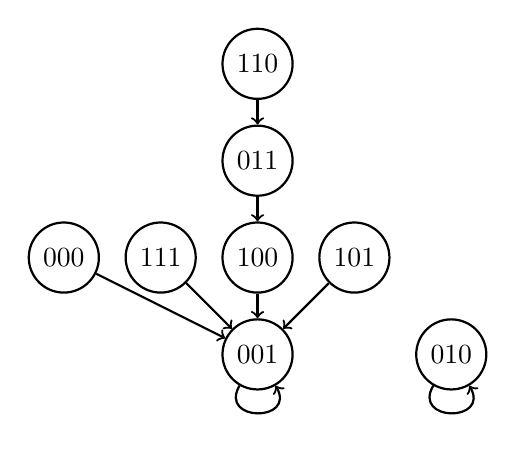
\begin{tikzpicture}[node distance={3.5em}, thick, main/.style = {draw, circle}]
    \node[main] (111) {$\state{111}$};
    \node[main] (000) [left of=111] {$\state{000}$};
    \node[main] (100) [right of=111] {$\state{100}$};
    \node[main] (001) [below of=100] {$\state{001}$};
    \node[main] (011) [above of=100] {$\state{011}$};
    \node[main] (110) [above of=011] {$\state{110}$};
    \node[main] (101) [right of=100] {$\state{101}$};

    \node[main] (010) [right of=001, xshift=3.5em] {$\state{010}$};

    \draw[->] (111) -- (001);
    \draw[->] (011) -- (100);
    \draw[->] (110) -- (011);
    \draw[->] (001) to [out=240, in=300, looseness=3] (001);
    \draw[->] (010) to [out=240, in=300, looseness=3] (010);
    \draw[->] (000) -- (001);
    \draw[->] (101) -- (001);
    \draw[->] (100) -- (001);
\end{tikzpicture}
\caption[An example of a STG]{An example of a state transition graph.}
\label{fig:STG}
\end{figure}
\end{lexample}

In the above example, we can see an interesting feature. The STG contains two
states the system cannot escape from. Component $a$ is absent in both, and
either $b$ or $c$ is active. Moreover, all but one state leads to the final
state $\state{001}$ in the long term. We call them \emph{attractors}, with the
latter having a larger \emph{basin}.

\begin{ldefinition}
An \emph{attractor} of a boolean network $\BN{B}$ is a maximal (finite) set
of states $\attr{A} = \set{\nu_i}_{i=1}^k$ such that:
\[ \forall_{\nu_1, \nu_2 \in \attr{A}} : \nu_1 \BNtc{B} \nu_2 \]

A \emph{basin} of attractor $\attr{A}$ is a (finite) set of all states $\nu$
such that:
\[ \exists_{\nu^{'} \in \attr{A}} : \nu \BNtc{B} \nu^{'} \]
We slightly abuse the notation and write just $\nu \BNtc{B} \attr{A}$.
\end{ldefinition}

\begin{lexample}
For the STG depicted in figure~\ref{fig:STG}, the basin of attractor
$\set{\state{010}}$ is just $\set{\state{010}}$ and the basin of attractor
$\set{\state{001}}$ is a set of all the other vertices.
\end{lexample}


Attractors are categorized based on their size and transitions within. The
simplest case is an attractor containing just one node. It is called a
\emph{fixed-point} attractor. In any other case, the attractor is
\emph{cyclic}. Intuitively, the system cyclically transitions among the states
in a fixed order.

In a synchronous model of the mammalian cell cycle from 2004~\cite{mammalian},
the analysis revealed two attractors: a fixed-point one with a basin of
attraction corresponding to a lack of growth factors, leading to the phase G0
or cell quiescence, and the second one cyclic attractor qualitatively matching
the data and simulation of Novak and Tyson~\cite{novak}. But the synchronous
approach prohibits further refined analysis of the transitions in the cyclic
attractor.

For asynchronous update policy, the categorization is more complex, rising from the fact that the STG contains more edges. Still, the fixed-point attractors coincide with the ones for synchronous policy~\cite{attractors}.

Although T.~Parmer~et~al.~\cite{infl_max_BN} have tried various update
policies, the synchronous one was used to obtain the results presented in their
article that we build on.  It seems to be the most straightforward as well, in
connection to the approximation algorithm they presented. We elaborate more on
this in the next chapter. The article also states that their method, as it is
currently designed, is not usable for cyclic attractors:
\blockquote[T.~Parmer~et~al.~\cite{infl_max_BN}]{Finally, as it is currently
formulated, our method is useful for the study of fixed points only but not
of limit cycles. The method can be generalized to the study of these more
complicated attractors, but only via a non-trivial generalization of our
currently proposed metric of dynamical influence.}

To put it together:
\begin{itemize}
    \item Synchronous semantics leads to simpler STG for analysis.
    \item There is evidence that fixed-point attractors have a more apparent
        analogy to the biological phenotype.
    \item Fixed-point attractors are the same for synchronous and asynchronous
        semantics.
    \item The stimulating article for our thesis works with fixed-points in
        synchronous update policy.
\end{itemize}
Thus we have chosen to focus only on fixed-point attractors and synchronous
semantics.

\subsection{Control of boolean networks}

To ensure that a boolean network reaches a specific, wanted attractor, one has
to interfere with the system if its state transition graph contains multiple
attractors. Such interference is called \emph{perturbation} or \emph{control}.
Two kinds of perturbations exist: state perturbations and update function
perturbations. In the former case, one changes the system's state or restricts
its state space. In the latter case, the STG edges are manipulated by adjusting
the update functions. Usually, it is much less realistic to change a biological
process than to change a system's state, e.g., by adding some
substance~\cite{zanudo}. Therefore we speak only about state perturbations.

State perturbations can be categorized in the following
way~\cite{smijakova_thesis}:
\begin{description}
    \item[One-step] Applied only once, then the system evolves freely due to
        the update policy and functions.
    \item[Temporary] Applied in multiple consequent time steps.
    \item[Permanent] The state space is restricted forever. For example, a
        chosen component cannot be active at all.
\end{description}

\begin{lexample}
When the system in Figure~\ref{fig:STG} settles down in state $\state{010}$
but we would like to have it in the other attractor, $\state{001}$, a
simple one-step control is to change component $a$ to a high state.
Afterward, the system progressively moves from state $\state{110}$ to
$\state{001}$ without any other perturbation because $\state{110}$ lies
in the basin of attraction for $\state{001}$.
\end{lexample}

In our thesis, we are interested in permanent control. It is the most intrusive
and unrealistic one, as it requires forever adding or extracting the
corresponding substance. But, again, the choice has been made regarding the
article~\cite{infl_max_BN} we build on, where the authors work with permanent
perturbations. The control is given by a \emph{driver-set} that drives the
system toward a specific attractor.

\begin{ldefinition}
A \emph{driver-set} $\dset{D}$ for a BN $\BN{B}$ with variables $V$ is a
restriction of (total) valuation $V \to \set{0, 1}$. After application of
$\dset{D}$, the state transition graph $\stg(B)$ is transformed subsequently:
\begin{itemize}
    \item Its vertices are reduced to $V' = \set{\nu \mid \dset{D} \text{ is
        a restriction of } \nu}$. We remind that a function $f$ is a
        restriction of $g$, when:
        \[
        \dom{f} \subseteq \dom{g} \land \forall_{x \in \dom{f}} : f(x) = g(x)
        \]
    \item The edges starting not from $V'$ are removed.
        Each remaining edge $(\nu_{\text{fr}}, \nu_{\text{to}})$ is
        substituted by an edge $(\nu_{\text{fr}}, \nu_{\text{to}}')$,
        such that
        \[
            \nu_{\text{to}}'(v) =
            \begin{cases}
                \dset{D}(v) & \text{if } v \in \dom{\dset{D}},\\
                \nu_{\text{to}}(v) & \text{else}.
            \end{cases}
        \]
        for all $v \in V$. ($\dom{f}$ denotes a domain of a function $f$.)
\end{itemize}

$\dset{D}$ can be interpreted also as a set of $\BN{B}$'s variable
\enquote{fixes}
\[
    \set*{(v, s) \mid v \in V \land s \in \set{0, 1}}.
\]
\end{ldefinition}

\begin{lexample}
Possible driver-sets for the BN defined in Example~\ref{example:BN} are:
$\dset{D_1} = \set{(b, 1)}$, $\dset{D_2} = \set{(b, 1), (c, 0)}$,
or $\dset{D_3} = \set{(b, 0)}$. We depict the related transformations of the STG
in Figure~\ref{fig:STG_transformed} (see the original STG in
Figure~\ref{fig:STG}). $\dset{D_1}$ is not enough to drive the system to
the attractor $\state{010}$ from any state. Adding $(c, 0)$ results in
$\dset{D_2}$ and transforms the $\stg{B}$ to have only one attractor. On the
other side, a driver set $\dset{D_3}$ of size 1 is sufficient to drive the
system toward the other attractor $\state{001}$.
\begin{figure}[!ht]
\centering
\begin{subfigure}{0.3\textwidth}
    \centering
    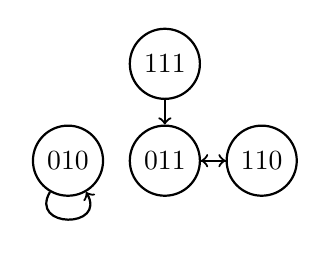
\begin{tikzpicture}[node distance={3.5em}, thick, main/.style = {draw,
                        circle}]
        \node[main] (111) {$\state{111}$};
        \node[main] (011) [below of=111] {$\state{011}$};
        \node[main] (110) [right of=011] {$\state{110}$};

        \node[main] (010) [left of=011] {$\state{010}$};

        \draw[->] (111) -- (011);
        \draw[->] (011) -- (110);
        \draw[->] (110) -- (011);
        \draw[->] (010) to [out=240, in=300, looseness=3] (010);
    \end{tikzpicture}
    \caption{$\set{(b, 1)}$}
\end{subfigure}
\hfill
\begin{subfigure}{0.3\textwidth}
    \centering
    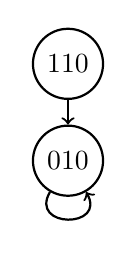
\begin{tikzpicture}[node distance={3.5em}, thick, main/.style = {draw,
                        circle}]
        \node[main] (110) {$\state{110}$};

        \node[main] (010) [below of=110] {$\state{010}$};

        \draw[->] (110) -- (010);
        \draw[->] (010) to [out=240, in=300, looseness=3] (010);
    \end{tikzpicture}
    \caption{$\set{(b, 1), (c, 0)}$}
\end{subfigure}
\hfill
\begin{subfigure}{0.3\textwidth}
    \centering
    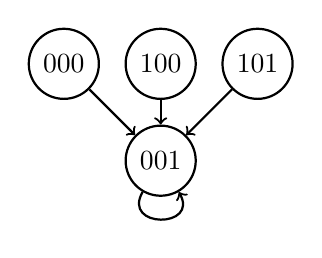
\begin{tikzpicture}[node distance={3.5em}, thick, main/.style = {draw,
                        circle}]
        \node[main] (000) {$\state{000}$};
        \node[main] (100) [right of=000] {$\state{100}$};
        \node[main] (001) [below of=100] {$\state{001}$};
        \node[main] (101) [right of=100] {$\state{101}$};

        \draw[->] (001) to [out=240, in=300, looseness=3] (001);
        \draw[->] (000) -- (001);
        \draw[->] (101) -- (001);
        \draw[->] (100) -- (001);
    \end{tikzpicture}
    \caption{$\set{(b, 0)}$}
\end{subfigure}
\caption{Resulting STGs after a control of given driver-sets.}
\label{fig:STG_transformed}
\end{figure}
\end{lexample}


% TODO is this neccessary?
%\makeatletter\thesis@blocks@clear\makeatother
%\phantomsection %% Print the index and insert it into the
%\addcontentsline{toc}{chapter}{\indexname} %% table of contents.
%\printindex

\appendix
\chapter{An appendix}
Here you can insert the appendices of your thesis.

\end{document}
